\chapter{Estimating Defect Probabilities} \label{chap:chap3}

\section*{}

In order to estimate the defect probabilty of each software component we developed a data mining application, agnostic to the project's language. 
It automatically extracts data from the current state and about older defects from a \emph{Git} repository, creates a model and predicts the probability. The project is written in Javascript (Node.js) and Python 3 and heavily uses \emph{node-git}
and \emph{scikit-learn}.

In this chapter, we will explain the concept behind it, approach the process used in each of the steps and will explain as how to install and use this application.

\subsection{Concept}

We assume that the patterns found in the components changed in older fix commits can help us determine present defective components. 
So, for a given repository state, we must identify the fix commits and the components changed in them, which are considered faulty.
Then for each fix commit the information about the components' state before the change must be extracted, as well as the information about the current state of each component.

Since the application should be able to predict the defect probability for any given software project that uses \emph{Git}, static analysis must not used. 
The only information that can be used is related to the file changes, authors, number of lines or bytes.

After the extraction, a machine learning model, created using the information about past defects, should predict the defect probability of each component present in the current state of the project.

% CHOURIÇO: Explaining image

\subsection{Main difficulties}

% **Difficulties**
% Accuracy now vs future
% Noisy commit messages
% Uncertantity about the clean/buggy stated used to train
% Language Agnostic

\subsection{Install}

The application relies on \emph{Redis}, \emph{Git}, \emph{Node.js} and \emph{Python 3} and requires some dependencies such as \emph{SciPy}, \emph{scikit-learn}, \emph{numpy}.

\begin{lstlisting}
  $ git clone --depth 1 https://github.com/atduarte/master-thesis.git
  $ cd master-thesis/app
  $ npm install --prod
\end{lstlisting}

\subsection{Usage}

After all the dependencies installed the usage is very straight-forward.
In order to automatically execute all the steps (extraction, data preparation, modeling and prediction) the following command should be used
by replacing "\code{{project-name}}" and "\code{{repository-path}}" respectively with
the chosen project name and the path to the folder containing the repository we want to analyze:

\begin{lstlisting}
  $ node index.js all {project-name} {repository-path}
\end{lstlisting}

It's possible to specify a diferent classification label (e.g. "\code{--classification-label=_mostChanged}", default is "\code{_mostChanged25}"), 
a different number of estimators used when modeling (e.g. "\code{--estimators=100}", default is 5) or even
to define the level of logging by appending, for example, "\code{--log-level=verbose}". The existing levels available, from higher to lower priority, are
"\code{error}", "\code{warn}", "\code{info}", "\code{verbose}" and "\code{silly}". The default log level is "\code{info}".

\begin{lstlisting}[style=npmlog]
  ?$  node index.js all math ../../tests/Math001?
  @info@ !extract/extract! Raw Extraction started
  @info@ !extract/extract! 499 fix commits found
  @info@ !prepareJson/prepare! JSON Preparation started
  @info@ !prepareJson/prepare! Will prepare 639 files
  @info@ !results/prepare! CSV Preparation started
  @info@ !results/prepare! Got 552 files
  @info@ !results/prepare! Got 203 columns
  @info@ !results/ml! Modeling
\end{lstlisting}

Some extra configurations are also available by creating a project configuration file, in the folder "\code{project-config/}", with the same name as the \code{project-name} plus ".js".
It allows to change the \emph{regex} used to identify the fix commits, to define a file filter and to define an email normalizer, in order to improve the quality of the extracted data .

\begin{lstlisting}[language=Javascript]
  'use strict';

  module.exports = {
      fileFilter: (filename) => {
          filename = filename.toLowerCase();

          return filename.endsWith('.java') // Is Java
              && !filename.startsWith('src/test'); // Aren't tests
      },
  };
\end{lstlisting}

Before terminating, the application will create a file ("\code{prediction.e500._mostChanged25.csv}", by default) in the repository folder containing the predicted defect probability for each source code file.

\begin{lstlisting}
  ...
  src/main/java/org/joda/time/Chronology.java,0.0
  src/main/java/org/joda/time/DateMidnight.java,0.21
  src/main/java/org/joda/time/DateTime.java,0.484
  src/main/java/org/joda/time/DateTimeComparator.java,0.0
  src/main/java/org/joda/time/DateTimeConstants.java,0.0
  src/main/java/org/joda/time/DateTimeField.java,0.006
  src/main/java/org/joda/time/DateTimeFieldType.java,0.002
  src/main/java/org/joda/time/DateTimeUtils.java,0.966
  src/main/java/org/joda/time/DateTimeZone.java,0.414
  src/main/java/org/joda/time/Days.java,0.0
  ...
\end{lstlisting}

% CHOURIÇO: Example of metadata information

In order to be able to execute only some step of the process, there's the possibility of executing only one operation. The available commands are:
%
\begin{itemize}
\item "\code{raw}" - Extracts data from \emph{Git} and saves it to "\code{out/{project-name}/raw}"
\item "\code{json}" - Processes the raw data and converts it to a new JSON structure. Results are saved to "\code{out/{project-name}/json}"
\item "\code{results}" - Creates the CSV files for training and prediction data, based on the JSON files, creates the model and predicts the defect probability.
Final result is saved at "\code{{repository-path}/prediction.csv}".
\end{itemize}

\subsection{Process}

As stated before the process is divided in extraction, data preparation, modeling and prediction steps. We will now dive deep into each.

\subsubsection{Extraction}

The first objective is to get the list of commits to analyze: the HEAD commit and all the fix commits that preceded it. 
So, first, the \emph{HEAD} commit is identified. The application then walks recursively through each parent commit or commits and,
if it's message matches the defined regex, doesn't contain any word from the stop words list, such as "typo" or "javadoc", and it isn't a merge, adds it to the list of commits to analyze.

% TODO: REGEX EXEMPLO

Having this list, it analyzes each commit individually, ignoring the ones that were already extracted or that have no changed files after filtering
according to configuration.
First the information directly related to the commit and it's tree is extracted:
%
\begin{itemize}
\item id - Id
\item message - Message
\item date - Date
\item author - Author
\item components - List of components
\end{itemize}

Then, the application walks through the changes history of each component, following name changes and extracting this info for each commit:
%
\begin{itemize}
\item id - Id
\item date - Date
\item author - Author
\item parentCount - Parent count
\item isFix - Is it a fix?
\item filename - Filename
\item lines - Number of lines
\item byteSize - Size of file in bytes
\item linesAdded - Number of lines added
\item linesRemoved - Number of lines removed
\end{itemize}

Since this procedure has a high computation cost, some enhancements have been made. It relies heavily on \emph{Redis} for caching 
and the number of components analyzed is reduced when possible. Considering that the modeling step will balance the training data, 
reducing the number of \emph{clean} components according to the number of existing \emph{buggy} components, the system randomizes the list and
limits the extraction of \emph{clean} components up to a maximum of four times the number of \emph{buggy} components on the given commit.

% TODO: Formula representing the maximum number o components?

% CHOURIÇO: Explain cache details

This data is then saved to a file named according to the commit id, in the "\code{raw}" folder (e.g "\code{out/math/raw/17d6f2163db436518f953166c1e9d495232f90b6}").

\begin{lstlisting}
  {
    "id": "0b1b9a9dc86da871ce5e7839b1b2df13c99dd9f8",
    "message": "Submitted Javadoc fixes from Andreou Andreas ...",
    "date": 1055343030,
    "author": "tobrien@apache.org",
    "components": {
      "src/java/org/apache/commons/math/ContractableDoubleArray.java": {
        "linesAdded": 3,
        "linesRemoved": 3,
        "changes": [
          {
            "id": "8b62ed457040b6a1b4562aa0d0df88e1e77bddce",
            "date": 1053499586,
            "author": "tobrien@apache.org",
            "parentCount": 1,
            "isFix": false,
            "filename": "src/java/org/apache/commons/math/ContractableDoubleArray.java",
            "lines": 322,
            "byteSize": 12970,
            "linesAdded": 54,
            "linesRemoved": 3
          },
          ...
        ]
      }
    }
  }
\end{lstlisting}

% GUIDELINE

% Identifica Head commit
% Percorre todos os commits que existem para traz e identifica fixes
% Extrai dados do Head Commit e dos fix commits (max = 1000) 
% Fix commits que não tenham ficheiros que procuramos alterados, nao são analisados
% Em Fix commits -> Nº de componentes nao modificados que sao analisados = 4 * Nº de ficheiros alterados no commit
% Lista de cenas que saca?
% > Base info
% > additional info
% example

\subsubsection{Data Preparation}

This step is the simplest. The only task is to convert the raw JSON structure, focused on the commit, to a JSON structure, focused on the component. 7
Iterating through each file at the "\code{raw}" folder and creating a new one with the same name in the "\code{json}" folder.

The data contained in this new file will be ready for being converted to CSV and to be used for modeling or prediction.

The following columns are prepared for each component:
%
\begin{itemize}
\item \_\_changed - Was it changed?
\item \_\_filename - Component name
\item \_lines - Number of lines
\item \_bytes - File size in bytes
\item \_mostChanged - Was it the most changed file in this commit?
\item \_mostChanged25 - Was this file in top 25\% of most changed files is this commit?
\item \_mostChanged50 - Was this file in top 50\% of most changed files is this commit?
\item \_mostChanged75 - Was this file in top 75\% of most changed files is this commit?
\item changes - Number of changes made in the past
\item changes:date-weighted - Sum of the result of the time-weighted function applied to each change
\item changes:size-weighted - Sum of the number of lines added and removed in each change
\item changes:date+size-weighted - Sum of the result of the time-weighted function applied to each change multiplied for the number of lines added and removed in it
\item authors - Number of authors that changed this file
\item authorChanges::{author} - Number of changes made in the past by a specific author. E.g. authorChanges::luc@apache.org
\item authorChanges:date-weighted:{author} - Sum of the result of the time-weighted function applied to each change made by a specific author. E.g. authorChanges:date-weighted::luc@apache.org
\item authorChanges:size-weighted:{author} - Sum of the number of lines added and removed in each change made by a specific author. E.g. authorChanges:size-weighted::luc@apache.org
\item authorChanges:date+size-weighted:{author} - Sum of the result of the time-weighted function applied to each change made by a specific author multiplied for the number of lines added and removed in it. E.g. authorChanges:date+size-weighted::luc@apache.org
\end{itemize}

% TODO: Time-Weighted Function

In order to improve modeling results, we also created the columns "changes-others", "changes-others:date-weighted", "changes-others:size-weighted", "changes-others:date+size-weighted", 
"changes-fixes", "changes-fixes:date-weighted", "changes-fixes:size-weighted" and "changes-fixes:date+size-weighted" that are equal to the already existing columns starting with
"changes", but refer only to changes that were not fixes and changes that were fixes, respectively.

Ploting the results we noticed that the date influenced significantly the data related to changes, since older commits have less history behind. 
So for each, we added a normalized version by the commit.

\begin{figure}[H]
  \begin{center}
    \leavevmode
    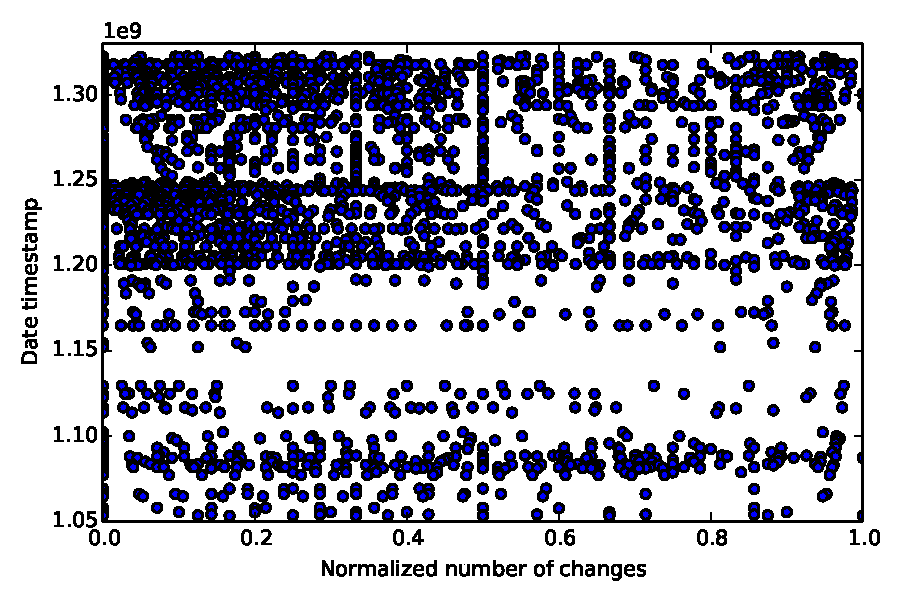
\includegraphics[width=0.75\textwidth]{date-changes_norm_math001.pdf}
    \caption{Example of the influence of the date on number of changes. (Project Math, Defect 1)}
    \label{fig:date-changes.raw}
  \end{center}
\end{figure}

\begin{figure}[H]
  \begin{center}
    \leavevmode
    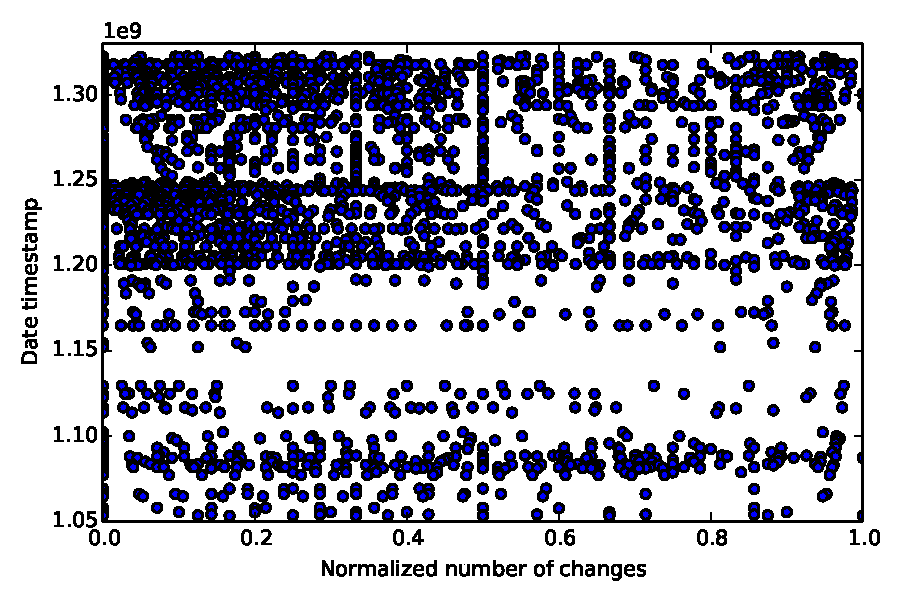
\includegraphics[width=0.75\textwidth]{date-changes_norm_math001.pdf}
    \caption{Example of the relation between the date on the normalized number of changes. (Project Math, Defect 1)}
    \label{fig:date-changes.norm}
  \end{center}
\end{figure}

\begin{lstlisting}
[
  {
    "__changed": true,
    "__date": 1364521362,
    "__filename": "src/main/java/org/apache/commons/math3/distribution/fitting/MultivariateNormalMixtureExpectationMaximization.java",
    "_lines": 441,
    "_bytes": 18211,
    "_mostChanged": false,
    "_mostChanged25": true,
    "_mostChanged50": true,
    "_mostChanged75": true,
    "changes:raw": 3,
    "changes:normalized": 0.2857142857142857,
    "changes-fixes:raw": 0,
    "changes-fixes:normalized": 0,
    "changes-others:raw": 3,
    "changes-others:normalized": 0.3333333333333333,
    "changes:date-weighted:raw": 2.979453,
    "changes:date-weighted:normalized": 0.290809968305134,
    "changes:size-weighted:raw": 481,
    "changes:size-weighted:normalized": 0.4746494066882416,
    "changes:date+size-weighted:raw": 477.701982,
    "changes:date+size-weighted:normalized": 0.4831911672918317,
    "changes-fixes:date-weighted:raw": 0,
    "changes-fixes:date-weighted:normalized": 0,
    "changes-fixes:size-weighted:raw": 0,
    "changes-fixes:size-weighted:normalized": 0,
    "changes-fixes:date+size-weighted:raw": 0,
    "changes-fixes:date+size-weighted:normalized": 0,
    "changes-others:date-weighted:raw": 2.979453,
    "changes-others:date-weighted:normalized": 0.3394176672358086,
    "changes-others:size-weighted:raw": 481,
    "changes-others:size-weighted:normalized": 0.4845814977973568,
    "changes-others:date+size-weighted:raw": 477.701982,
    "changes-others:date+size-weighted:normalized": 0.49340824785460163,
    "authors:raw": 3,
    "authors:normalized": 0.6666666666666666,
    "authorChanges::luc@apache.org:raw": 1,
    "authorChanges::luc@apache.org:normalized": 0,
    ...
    "authorChanges:date-weighted::luc@apache.org:raw": 0.993164,
    "authorChanges:date-weighted::luc@apache.org:normalized": 0.00025474141229450394,
    "authorChanges:size-weighted::luc@apache.org:raw": 33,
    "authorChanges:size-weighted::luc@apache.org:normalized": 0.5454545454545454,
    "authorChanges:date+size-weighted::luc@apache.org:raw": 32.774417,
    "authorChanges:date+size-weighted::luc@apache.org:normalized": 0.5455704368440787,
    ...
  },
  ...
]
\end{lstlisting}
\caption{Example of extracted data}


The data from the multiple fix commits is then combined in a file named "history.csv" and the data from the \emph{HEAD} commit is placed at "master.csv". 
These two files will be only files required to execute the next step.


\subsubsection{Modeling and Prediction}

For modeling and predicting \emph{Python 3} and \emph{scikit-learn} is used.
Random Forests, Decision Trees and Naive Bayes were tried, but the former achieved significantly better results as it's presented in the Experimental Results chapter \ref{chap:exp-res}.
Neural Networks weren't used since the training set is normally small.

Before training the model, the training set is randomized and balanced, first to a ratio of 5 \emph{clean} component for each \emph{buggy} component 
and then SMOTE is used to create more \emph{buggy} component entries. In order to train the model a \emph{Stratified KFold} (4 folds) is used and run 10 times, 
generating 40 different models. Performance of these 40 models is measured according to the difference of the mean defect probability of buggy test data and clean test data. 
The 15 models with the highest difference are then used to predict the defect probability of each component in the current project state and a mean is calculated.

As refered before, the results are saved directly at the repository folder.
